\documentclass{memo}
\usepackage{mathptm,mydef,myenv}
\usepackage[all]{xy}
\usepackage{graphicx}
%\usepackage{MinionPro}
\begin{document}
\small
\noindent{\large\bf{}Hadoop MapReduce Framework}

\paragraph{Overview}
A MapReduce {\em job\/} splits the input dataset into independent chunks
processed by {\em map\/} tasks in completely parallel manner, followe by {\em
  reduce\/} tasks which aggregates their output.  Typically both the input and
the output of the job are stored in a Hadoop {\tt FileSystem}. 

\paragraph{MapReduce inputs and outputs}
The MapReduce framework operates exclusively on $\arc{\mbox{\em key,
    value\/}}$ pairs. The {\em key\/}s and {\em value\/}s have to be
serializable as \verb+Writable+s and additionally the {\em key\/}s have to be
{\em WritableComparable\/}s in order to facilitate grouping by the framework. 

The following is an overall flow of a MapReduce Job:
\[
\xymatrix@-1.0pc{
  \arc{k_1, v_1} \ar[r] & \mbox{\bf map} \ar[r] & \arc{k_2, v_2} \ar[r] & 
  \mbox{\bf combine} \ar[ld] \\
 \arc{k_3, v_3} &
  \mbox{\bf reduce} \ar[l]  &
  \arc{k_2, v_2} \ar[l] \\
}
\]

\paragraph{Hadoop mapper}
The mapper takes input $\arc{\mbox{\em key, value}}$ pairs, perform
computation, and generates a set of
intermediate $\arc{\mbox{\em key, value}}$ pairs. 

\begin{verbatim}
  map(KEYIN key,Iterable<VALUEIN> values,
      Mapper.Context ctx);

  public class WordCount {
    public static class Map 
      extends Mapper<LongWritable, Text, 
                     Text, IntWritable> {
      public void map(LongWritable key, 
                      Text value,
                      Context context) {
        String line = value.toString();
        StringTokenizer tk = new ...(line);
        while (tk.hasMoreTokens()) {
          word.set(tk.nextToken());
          context.write(word, one);
  }}}}
\end{verbatim}

\paragraph{Hadoop reducer}
The Hadoop reducer reduces a set of intermediate values {\em which share
  a key\/} to a (usually smaller) set of values. 

A {reducer} has three primary phases: {\em shuffle\/}, {\em sort\/}, and
{\em reduce\/}. In the \bb{shuffle} phase, input to the {\tt Reducer} is
sorted output of the mappers. In this phase, the framework fetches the
relevant partition of the output of all the mappers, via HTTP. In the
\bb{sort} phase, the framework groups {\tt Reducer} inputs by keys in this
phase (since different mappers may have output the same key). 
At the \bb{reduce} phase, the {\tt reduce()} method is called for each 
$\arc{\mbox{\em key, list of values}}$ pair in the grouped inputs. 
\begin{verbatim}
  reduce(KEYIN key,Iterable<VALUEIN> values,
         Reducer.Context ctx);

  public class WordCount {
    public static class Reduce 
      extends Reducer<Text, IntWritable, 
                      Text, IntWritable> {
      public void map(Text key, 
                      Iterable<IntWritable> values,
                      Context context) {
        int sum = 0;
        for (IntWritable val : values) {
          sum += val.get();
        }
        context.write(key, new IntWritable(sum));
      }
    }
  }
\end{verbatim}
The heart of {\tt Reducer} is its {\tt reduce()} method.  This method is
called {\em once per key\/}. The second argument is an {\tt Iterable/} which
returns all the values associated with the key. 

\paragraph{Running MapReduce jobs}

\begin{verbatim}
  public class WordCount {
    public int run(String[] args) {
      Job job = new Job(getConf());
      job.setJarByClass(WordCount.class);

      job.setOutKeyClass(Text.class);
      job.setOutValueClass(IntWritable.class);

      job.setMapperClass(Map.class);
      job.setCombinerClass(Reduce.class);
      job.setReducerClass(Reduce.class);

      job.setInputFormatClass(TextInputFormat);
      job.setOutputFormatClass(TextOutputFormat);
    }

    public static void main(String[] args) {
      ToolRunner.run(new WordCount(), args);
  }}
\end{verbatim}

\paragraph{How Hadoop runs a MapReduce job}
For a single MapReduce job, there four independent entities: {\em clinent\/},
{\em jobtracker\/}, {\em tasktracker\/}, and {\em HDFS\/}. 

\begin{quote}
% jpg for pdflatex
%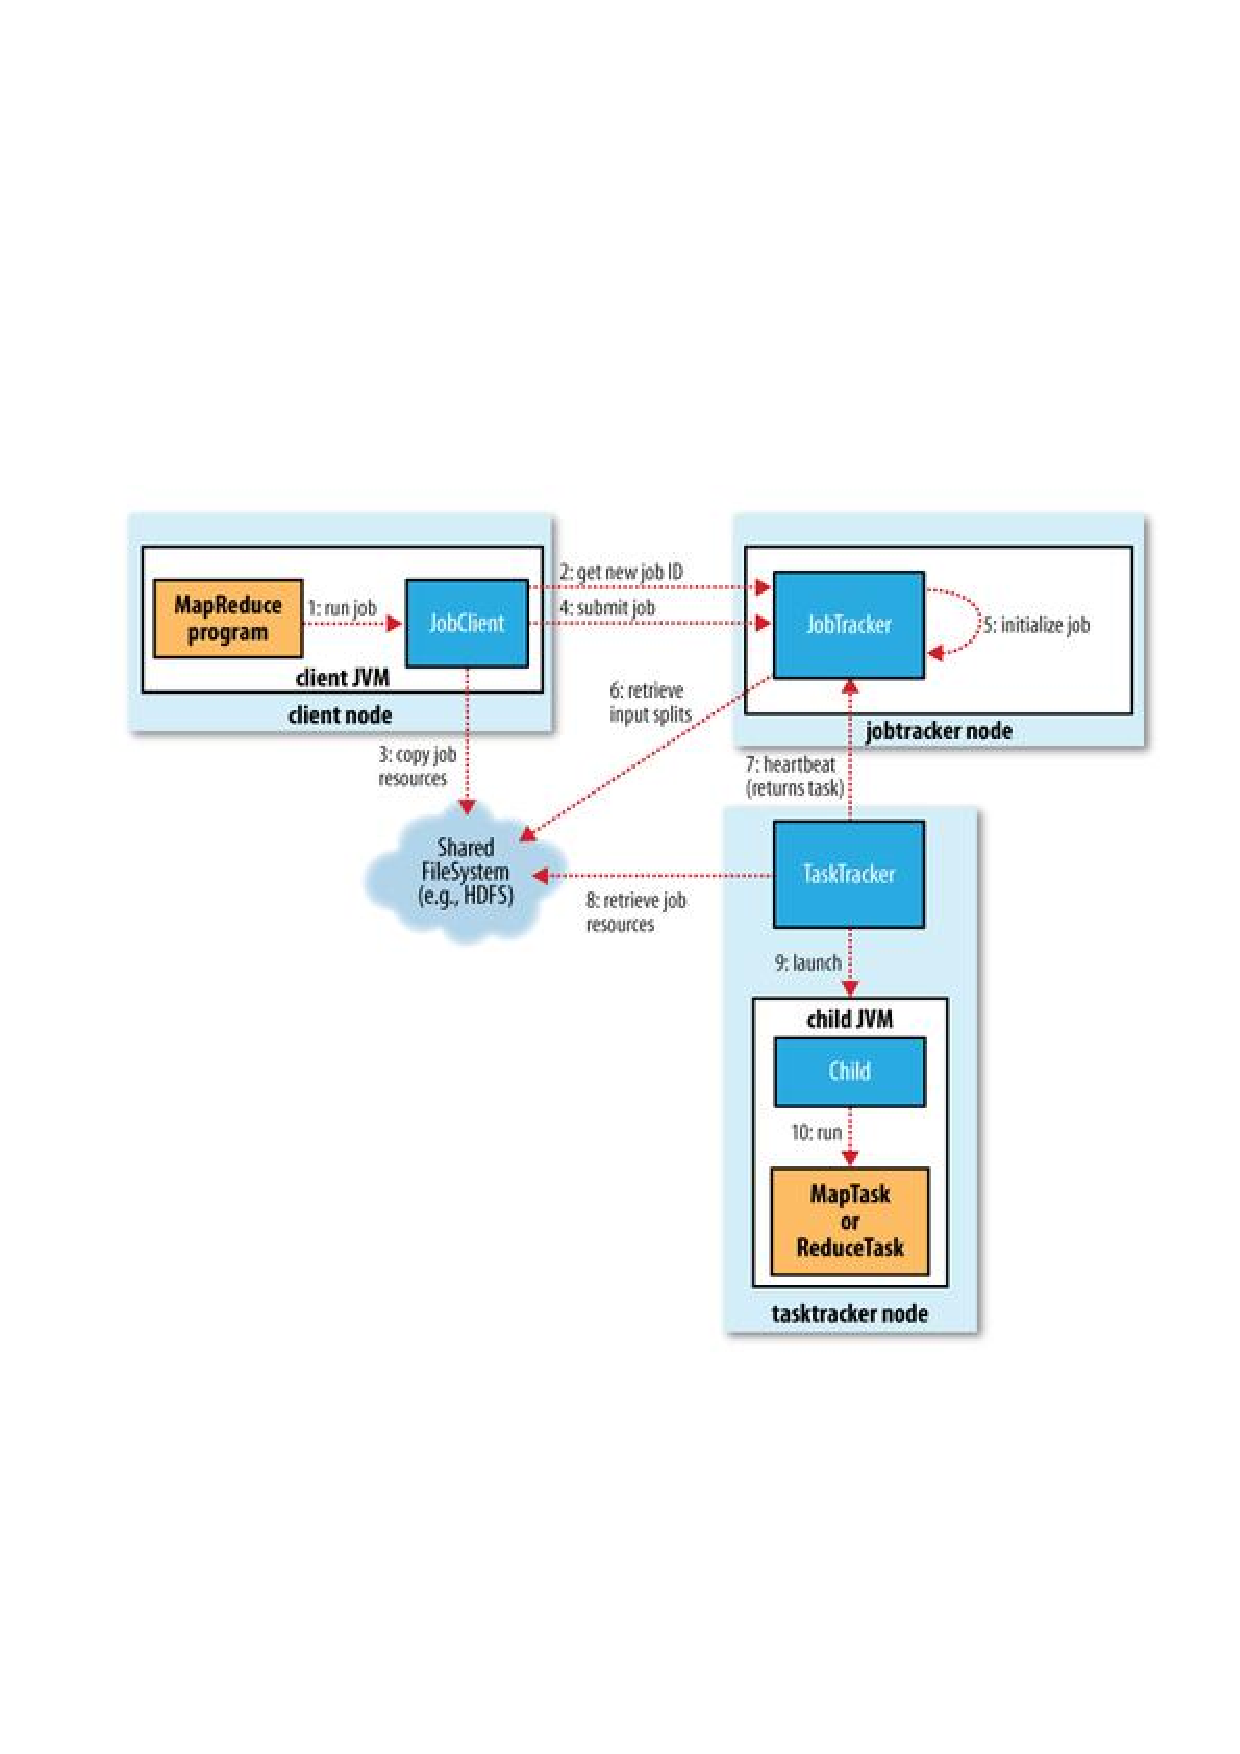
\includegraphics[scale=0.5]{mapred.jpg}
% ps for xdvi
\centerline{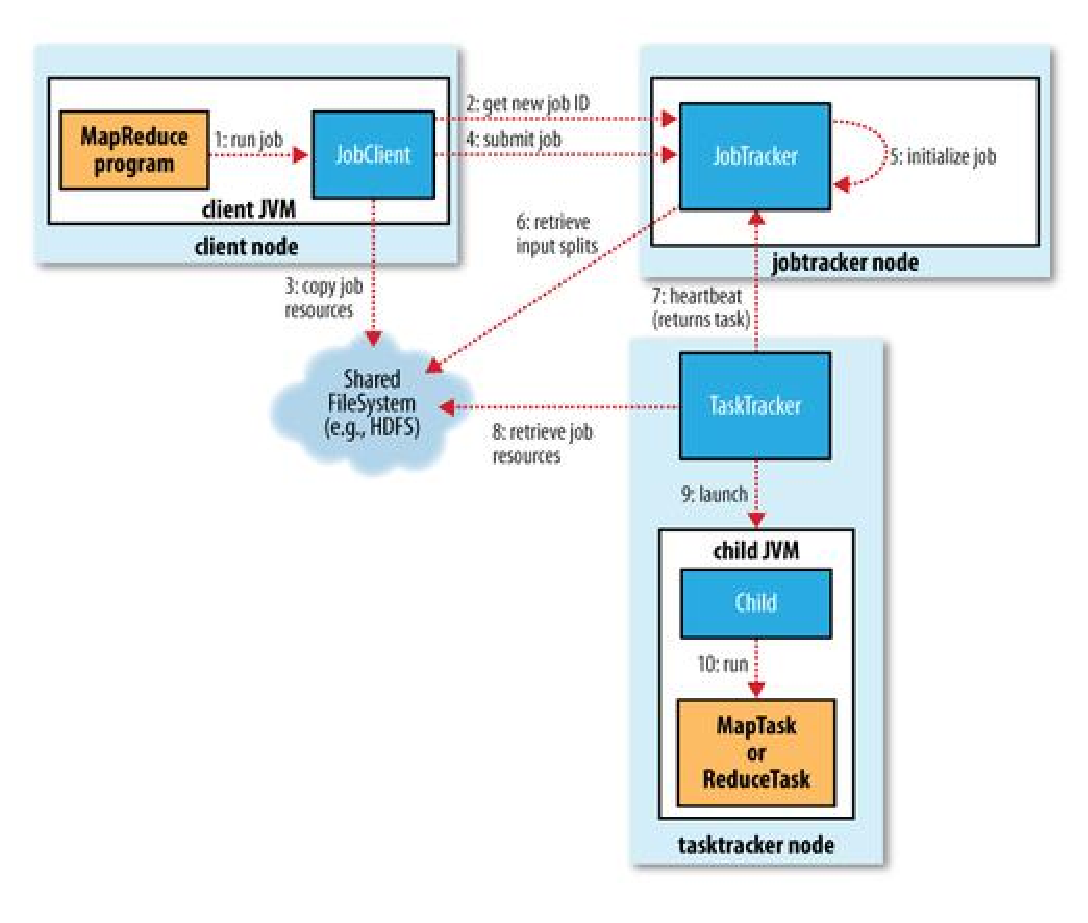
\includegraphics[scale=0.5]{mapred.ps}}
\end{quote}
\ben
\w (CLIENT) \bb{JobClient.runJob(conf)}:
  \ben
  \w create a new \bb{JobClient} instance
  \w call \bb{JobClient.submitJob()}
    \bit
    \w call \bb{JobTracker.getNewJobId()}: ask \bb{JobTracker} for a new Job
    ID
    \w check the output specification of the job (e.g. check if output
    directory was specified)
    \w compute {\em input splits\/} of the job 
    \w copies the resources needed to run the job (including i.e. \bb{job JAR}
      file (code), the configuration file, and the computed input splits to
        the jobtracker's filesystem in a directory named after the job ID
        
    \eit
  \w polls the job's progress once a second (and reports the progress to the
  console) 
  \w when job is complete or has failed, handle that approprately
  \een
\w (JOB-TRACKER) \bb{job initialization}: 
  \ben
  \w on \bb{JobTracker.submitJob()}, puts the job request into a \bb{job queue}
  \w later, \bb{job scheduler} will pick ths job from the queue and
  \bb{initialize} it
  \w initialization includes:
     \bit
     \w create an object that represwent the job being run, which encapsulates
     its tasks 
     \w create a list of {\em tasks\/} to run by creating one \bb{map task} for
     each input split
     \eit
  \een
\w (TASK-TRACKER) \bb{task assignment}:
  \ben
  \w run a simple loop that periodically sends \bb{heartbeat} method calls to
  the \bb{JobTracker} 
  \w 
  \een
\een

\end{document}

